\chapter{动物住在哪里}\label{ch:g2:where-animals-live}

你不会在校园里遇到鳟鱼，
也不会在池塘底部看到松鼠。每种\omterm{def:g1:animals-around-us:animal}{动物}都生活在适合它的地方——
那里有它的食物、庇护所和邻居。
生物学家为\omterm{def:g1:animals-around-us:animal}{动物}的家园取了一个名字。

\section{栖息地}

\begin{definition}[栖息地]\label{def:g2:where-animals-live:habitat}
\omterm{def:g1:animals-around-us:animal}{动物}的\emph{栖息地}\index{栖息地}是它自然生活的地方，
在那里它能找到所需的一切：
食物、水、庇护所，以及保护幼体的安全处所。池塘、
森林、草地、篱笆和海岸都是栖息地。
\end{definition}

\begin{example}[四种栖息地，四个邻里]\label{ex:g2:where-animals-live:four}
在\emph{池塘}里：青蛙、蜻蜓、刺鱼、池塘螺。
在\emph{森林}里：松鼠、鹿、啄木鸟、林蚁。
在\emph{草地}里：兔子、蚱蜢、蝴蝶、田鼠。
在老旧\emph{围墙}的石块下：潮虫、
蜘蛛，有时还有一只趴在顶上晒太阳的蜥蜴。
\end{example}

\begin{omfigure}
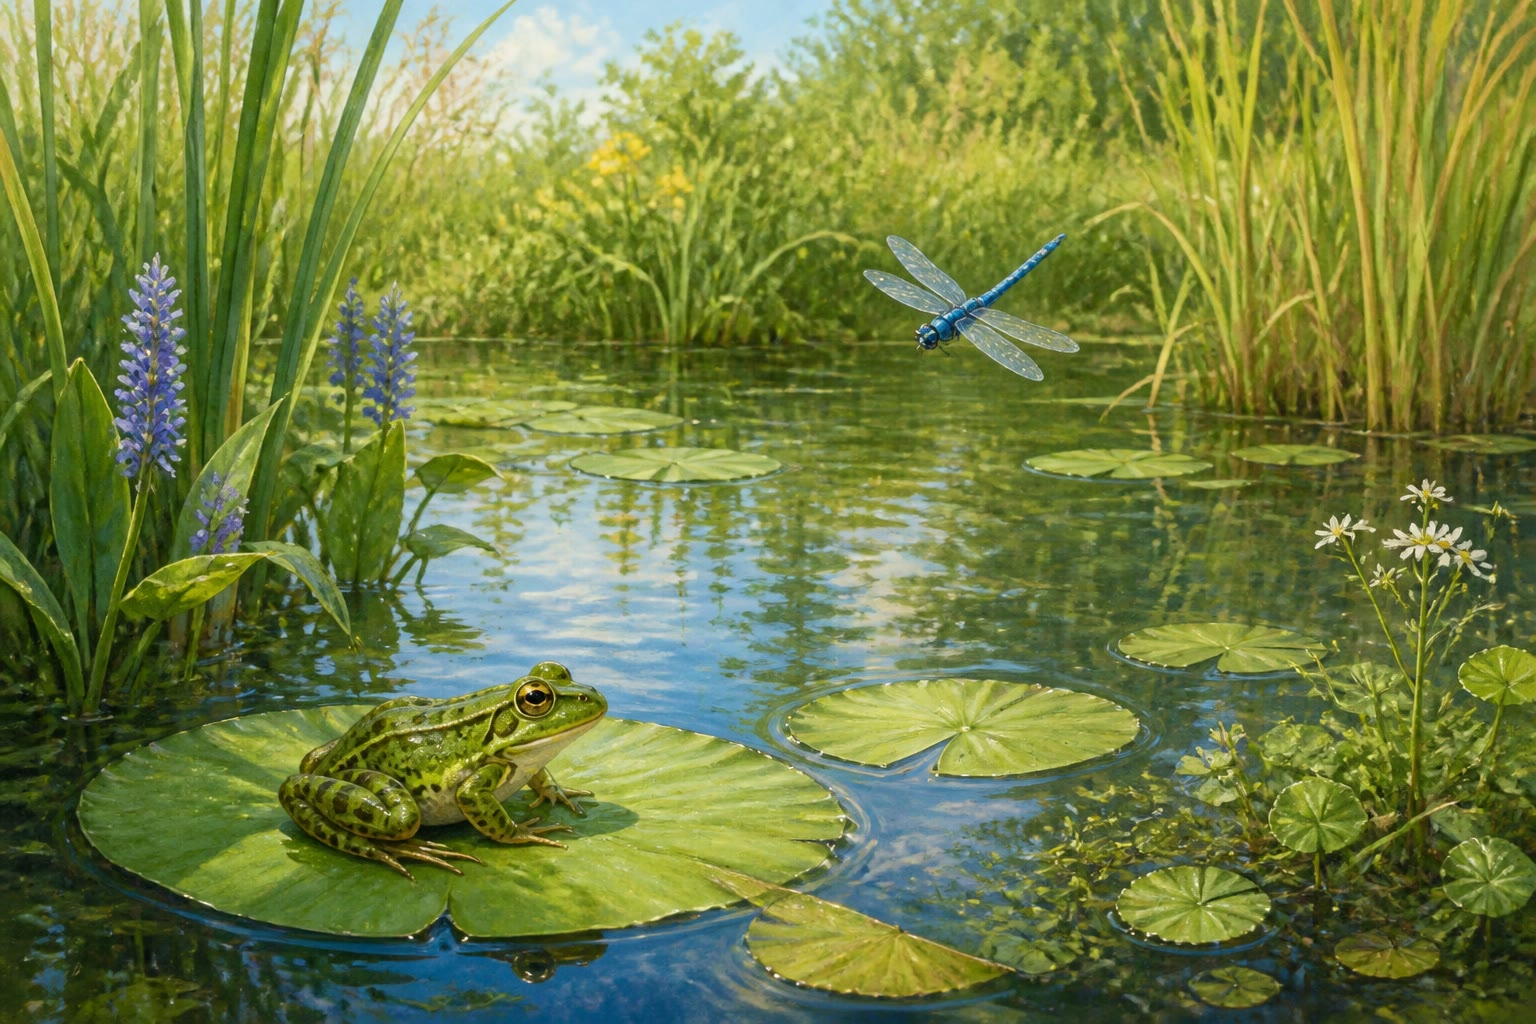
\includegraphics[width=0.62\linewidth]{images/book1/ai/g2-live-pond.jpg}

{\small 池塘\omterm{def:g2:where-animals-live:habitat}{栖息地}，两位住户在家：一只青蛙
蹲在睡莲叶上，一只蜻蜓在巡逻。}
\end{omfigure}

\begin{omfigure}
\begin{tikzpicture}[scale=0.88]
  \draw[thick, omDef, fill=omDef!7, rounded corners=6pt]
    (0,0) rectangle (3.4,2.6);
  \draw[thick, omMeth, fill=omMeth!7, rounded corners=6pt]
    (3.9,0) rectangle (7.3,2.6);
  \draw[thick, omProp, fill=omProp!7, rounded corners=6pt]
    (7.8,0) rectangle (11.2,2.6);
  \node[font=\small\bfseries, omDef] at (1.7,2.25) {池塘};
  \node[font=\small\bfseries, omMeth] at (5.6,2.25) {森林};
  \node[font=\small\bfseries, omProp] at (9.5,2.25) {草地};
  \node[font=\small, align=center] at (1.7,1.05)
    {青蛙 \\ 蜻蜓 \\ 刺鱼};
  \node[font=\small, align=center] at (5.6,1.05)
    {松鼠 \\ 啄木鸟 \\ 鹿};
  \node[font=\small, align=center] at (9.5,1.05)
    {兔子 \\ 蚱蜢 \\ 蝴蝶};
\end{tikzpicture}

{\small 三种\omterm{def:g2:where-animals-live:habitat}{栖息地}及其部分住户。试着互换它们
——松鼠在池塘里可住不了多久。}
\end{omfigure}

\begin{remark}[一个栖息地，许多住处]\label{rem:g2:where-animals-live:layers}
一个\omterm{def:g2:where-animals-live:habitat}{栖息地}有许多角落。同一片森林里，啄木鸟
住在高高的树干上，松鼠住在树枝间，鹿住在灌木丛中，
林蚁则住在地面上堆起的蚁巢里。
同一片森林，却有不同的楼层——所以许多\omterm{def:g1:animals-around-us:animal}{动物}
可以共享一个\omterm{def:g2:where-animals-live:habitat}{栖息地}而不致拥挤。
\end{remark}

\section{适应栖息地}

\begin{proposition}[动物与栖息地相适应]\label{prop:g2:where-animals-live:fit}
\omterm{def:g1:animals-around-us:animal}{动物}的身体和习性与它所生活的地方相适应：
\begin{itemize}
  \item 青蛙的蹼足能推水——它是为池塘而生的；
  \item 松鼠有抓握的爪子和粗大的平衡尾巴，
        是为树木而生的；
  \item 兔子有挖掘用的爪子和长长的警觉耳朵，
        是为有地洞的开阔草地而生的；
  \item 鸭子的\omterm{def:g1:animals-around-us:covering}{羽毛}能防水，它的蹼足
        能划水。
\end{itemize}
\omterm{def:g1:animals-around-us:animal}{动物}若被移到错误的\omterm{def:g2:where-animals-live:habitat}{栖息地}，就会失去这些优势。
\end{proposition}
\admitted

\begin{example}[鼹鼠的本领]\label{ex:g2:where-animals-live:mole}
鼹鼠生活在地下，住在它在草地下挖的隧道里。
它的前爪是宽大的挖掘铲，\omterm{def:g1:animals-around-us:covering}{皮毛}向两个方向都平顺贴伏，
因此泥土不会弄乱它的毛；它那弱小的眼睛
在黑暗中几乎派不上用场。在地面上它笨拙，
但在自己的\omterm{def:g2:where-animals-live:habitat}{栖息地}里，它是冠军。
\end{example}

\begin{method}[为动物匹配栖息地]\label{met:g2:where-animals-live:matching}
面对一种不认识的\omterm{def:g1:animals-around-us:animal}{动物}：
\begin{enumerate}
  \item 看看它的器官：有蹼足吗？有爪子吗？有翅膀吗？有挖掘用的
        前爪吗？
  \item 问问它吃什么，以及这些食物在哪里找到；
  \item 问问它在哪里能够躲藏并养育幼体；
  \item 能同时满足这三点的\omterm{def:g2:where-animals-live:habitat}{栖息地}，就是它最可能的家。
\end{enumerate}
\end{method}

\section{栖息地可能会丧失}

\begin{proposition}[没有栖息地，就没有住户]\label{prop:g2:where-animals-live:loss}
\omterm{def:g1:animals-around-us:animal}{动物}离开了\omterm{def:g2:where-animals-live:habitat}{栖息地}就无法生存。如果池塘被填平，
其中的青蛙和蜻蜓也会随之消失；如果篱笆被拔掉，
在那里筑巢的鸟就失去了庇护所。
保护\omterm{def:g1:animals-around-us:animal}{动物}，要从保护它们生活的地方开始。
\end{proposition}
\admitted

\begin{example}[学校的池塘]\label{ex:g2:where-animals-live:schoolpond}
一所学校在操场的一角挖了一个小池塘。
两年之内，蜻蜓在上面巡飞，水黾在水面上行走，
青蛙也搬了进来——没有人带它们来。
造好\omterm{def:g2:where-animals-live:habitat}{栖息地}，住户自然会找上门来。
\end{example}

\begin{remark}[不打扰地观察]\label{rem:g2:where-animals-live:respect}
参观\omterm{def:g2:where-animals-live:habitat}{栖息地}时，我们是客人。要安静地观察，
翻开的石头要照原样放回，不要触碰卵和巢，
垃圾要带回家，\omterm{def:g2:where-animals-live:habitat}{栖息地}应当察觉不到你曾经来过。
后面的章节会介绍更多照顾自然的方法。
\end{remark}

\section{练习}

\begin{exercise}[$\star$]\label{exo:g2:where-animals-live:1}
什么是\omterm{def:g2:where-animals-live:habitat}{栖息地}？说出\omterm{def:g1:animals-around-us:animal}{动物}在其中能找到的四样东西。
\end{exercise}

\begin{exercise}[$\star$]\label{exo:g2:where-animals-live:2}
分别举出池塘、森林和
草地中各两种\omterm{def:g1:animals-around-us:animal}{动物}。
\end{exercise}

\begin{exercise}[$\star$]\label{exo:g2:where-animals-live:3}
每种\omterm{def:g1:animals-around-us:animal}{动物}适合哪种\omterm{def:g2:where-animals-live:habitat}{栖息地}：三刺鱼、啄木鸟、
蚱蜢、鼠妇？
\end{exercise}

\begin{exercise}[$\star$]\label{exo:g2:where-animals-live:4}
青蛙的游泳工具是什么？松鼠的
爬树工具呢？
\end{exercise}

\begin{exercise}[$\star$]\label{exo:g2:where-animals-live:5}
列出鼹鼠的三种地下工具，
见\cref{ex:g2:where-animals-live:mole}。
\end{exercise}

\begin{exercise}[$\star$]\label{exo:g2:where-animals-live:6}
在\cref{rem:g2:where-animals-live:layers}中，
每种\omterm{def:g1:animals-around-us:animal}{动物}利用森林的哪一“层”：啄木鸟、松鼠、鹿、
林蚁？
\end{exercise}

\begin{exercise}[$\star$]\label{exo:g2:where-animals-live:7}
池塘被填平后，青蛙和蜻蜓会怎样？
这说明了保护\omterm{def:g1:animals-around-us:animal}{动物}的什么道理？
\end{exercise}

\begin{exercise}[$\star$]\label{exo:g2:where-animals-live:8}
试一试：在你家附近选一个小\omterm{def:g2:where-animals-live:habitat}{栖息地}，
比如石头下、灌木丛或花坛。安静地观察，在固定时间内
列出你看到的每一种\omterm{def:g1:animals-around-us:animal}{动物}。观察后把石头放回原处，
你的小\omterm{def:g2:where-animals-live:habitat}{栖息地}里住着多少个住户？
\end{exercise}

\begin{exercise}[$\star\star$]\label{exo:g2:where-animals-live:9}
一种神秘\omterm{def:g1:animals-around-us:animal}{动物}有蹼状的脚、能让水滑落的致密\omterm{def:g1:animals-around-us:covering}{羽毛}，
以及用来滤食的扁平喙。利用
\cref{met:g2:where-animals-live:matching}说出它的\omterm{def:g2:where-animals-live:habitat}{栖息地}，
也可以说出这种\omterm{def:g1:animals-around-us:animal}{动物}的名字。
\end{exercise}

\begin{exercise}[$\star\star$]\label{exo:g2:where-animals-live:10}
汤姆想“帮助”一只青蛙，把它带回家，
放进一个干燥、食物充足的玻璃饲养箱。利用
\cref{prop:g2:where-animals-live:fit}和
\cref{prop:g2:where-animals-live:loss}，解释为什么这样做
对青蛙毫无帮助。
\end{exercise}
